
\startslide{The Problem Setting: Embedded Sensor Networks}
\begin{center}
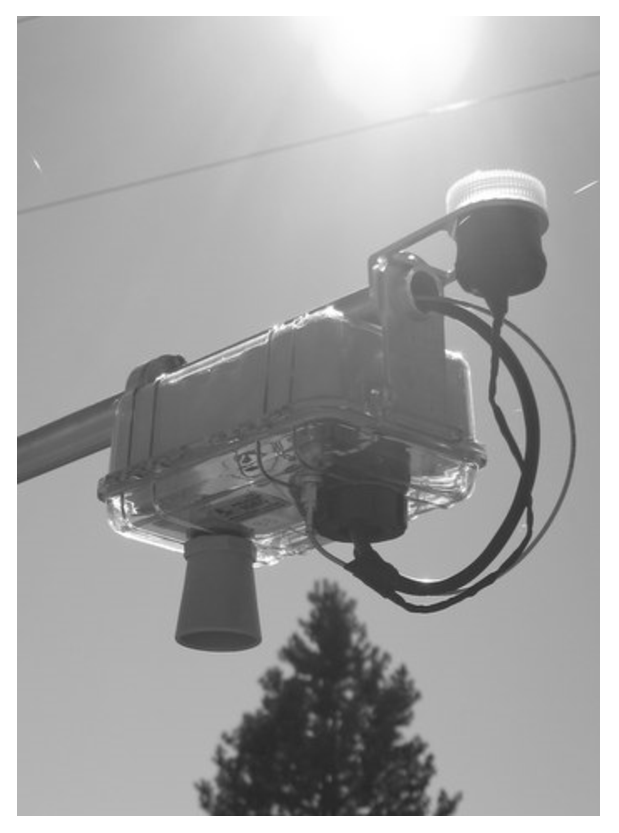
\includegraphics[scale=.50]{brainbox} 
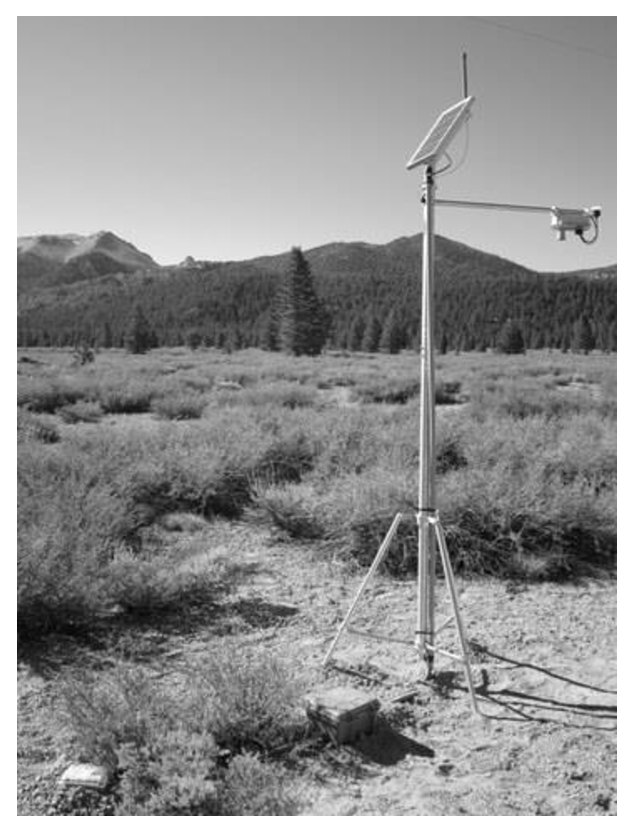
\includegraphics[scale=.50]{tower} 
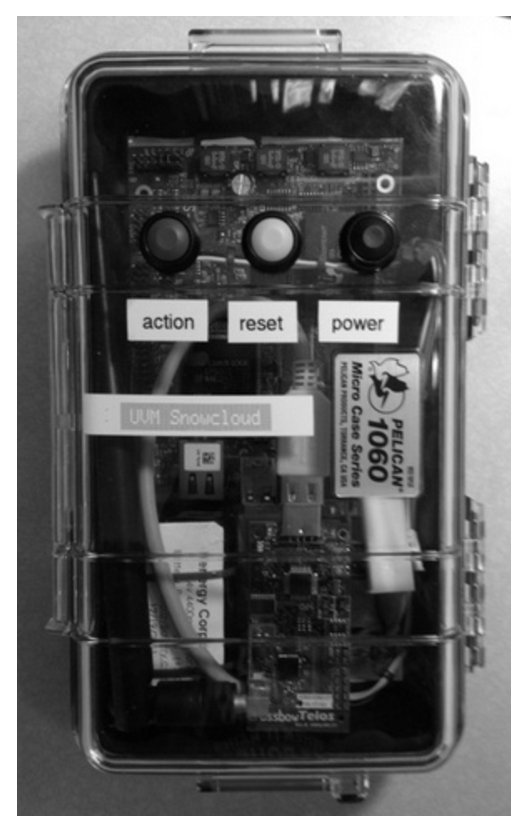
\includegraphics[scale=.50]{harvester} 
\end{center}

\begin{citemize}
\item Distributed data-gathering systems for earth and agricultural sciences.
\item At UVM, focus on alpine snow hydrology.
\begin{citemize}
\item Deployments in California, New Hampshire, Arctic Norway.
\end{citemize}
\end{citemize}
\stopslide

%%%%%

\startslide{Challenges of Programming Sensor Networks}
\begin{citemize}
\item Heavily resource constrained---RAM, ROM, clock cycles, power.
\item e.g., Crossbow TelosB: 4\,MHz, 10\,KiB RAM, 48\,KiB ROM
\item \ldots yet complex, distributed algorithms used.
\end{citemize}

State of the art:
\begin{citemize}
\item nesC and TinyOS: Optimized for efficiency, widely used.
\end{citemize}
\stopslide

%%%%%

\startslide{nesC Modules}
{\small
\begin{lstlisting}[language=nesC, escapechar=!]
#include "Message.h"              #include "Message.h"

module SendC {                    module RadioC {
  uses error_t radio_x(Msg*);       provides error_t radio_x(Msg*);
}                                   uses error_t handle_radio_r(Msg*);
implementation {                   }
  ...                              implementation {
}                                    ...
                                   }
\end{lstlisting} 
}
\begin{citemize}
\item Modules consist of a specification and implementation.
\item Specification lists used and provided \emph{commands}.
\item Implementation is a C-like translation unit.
\end{citemize}
\stopslide

%%%%%

\startslide{nesC Configurations}

{\small
\begin{lstlisting}[language=nesC]
               configuration AppC { }
               implementation {
                 components SendC, RadioC;
                 SendC.radio_x -> RadioC.radio_x;
               }
\end{lstlisting}
}

\begin{citemize}
  \item Application formed by \emph{wiring} components together.
  \item Component wiring is entirely static.
  \item Example above incomplete: unresolved import.
\end{citemize}
\stopslide

%%%%%

\startslide{Our Approach}
\begin{citemize}
\item \cemph{Staging with two stages}. Scala at metalevel, nesC residuum. Modules are the
  smallest unit of code manipulation.
\item Technical features: \cemph{Type specialization} with \cemph{dynamic type construction},
  \cemph{process separation}.
\item \cemph{Cross-stage type safety}: Type checking at Scala level ensures type safety of nesC
  residuum.
\item \cemph{Well-founded language design}.
\end{citemize}
\stopslide

%%%%%

\startslide{Workflow}
\centering
\scalebox{0.80}{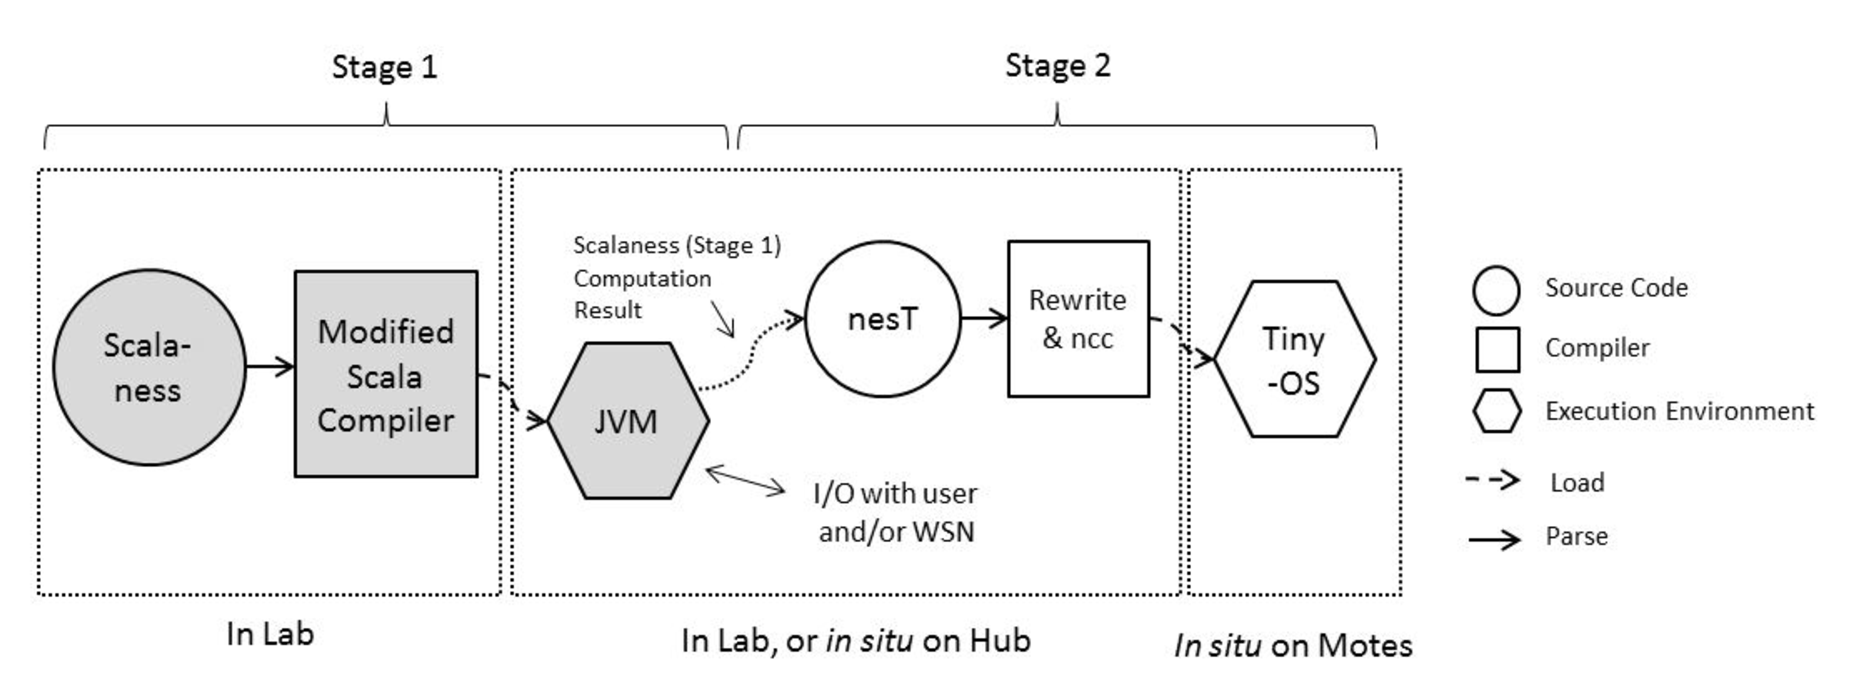
\includegraphics{scalaness}}
\begin{citemize}
\item \cemph{In the lab}: First stage program specializes and composes modules of second stage
  code.
\item \cemph{In the field}: Generated second stage program accounts for field conditions.
  Deployed to nodes (over the air).
\end{citemize}
\stopslide

%%%%%

\startslide{Example: Introducing Some Type Abbreviations}
\lstset{basicstyle=\ttfamily, escapeinside={(*@}{@*)}}
\begin{lstlisting}[language=nesC]
(*@\color{red}{\tt{abbrvt\ mesgT(t) =}}@*)
  (*@\color{red}{\tt\{ src : t; dest : t; data : uint8[] \};}@*)

(*@\tt{abbrvt\ radioT =}@*)
  < at (*@$\subtype$@*) uint32 >
  { export error_t radio_x((*@\tt{mesgT}@*)(at)*); 
    import error_t handle_radio_r((*@\tt{mesgT}@*)(at)*); };
\end{lstlisting}

\begin{citemize}
\item \color{red}{A record type parameterized by a type \tt{t}.}
\item \color{black}{nesT modules parameterized by types and values.}
\end{citemize}
\stopslide

%%%%%

\startslide{Example: Introducing Some Type Abbreviations}
\lstset{basicstyle=\ttfamily, escapeinside={(*@}{@*)}}
\begin{lstlisting}[language=nesC]
(*@\tt{abbrvt\ mesgT(t) =}@*)
  { src : (*@\tt{t}@*); dest : (*@\tt{t}@*); data : uint8[] };

(*@\color{red}{\tt{abbrvt\ radioT =}}@*)
  (*@\color{red}{\tt< at $\subtype$ uint32 >}@*)
  (*@\color{red}{\tt\{ export error\_t radio\_x(mesgT(at)*);}@*)
  (*@\color{red}{\tt\ \ import error\_t handle\_radio\_r(mesgT(at)*); \};}@*)
\end{lstlisting}

\begin{citemize}
\item A record type parameterized by a type \tt{t}.
\item \color{red}{nesT modules parameterized by types and values.}
\end{citemize}
\stopslide

%%%%%

\startslide{Example: nesT Modules}
\lstset{basicstyle=\ttfamily, escapeinside={(*@}{@*)}}
\begin{lstlisting}[language=nesC]
val (*@\tt{authSend =}@*)
  < at (*@$\subtype$@*) uint32; sendk : uint8[] >  
  { import error_t radio_x((*@\tt{mesgT}@*)(at)*);
    export error_t send(m : (*@\tt{mesgT}@*)(at)*) 
        { radio_x(AES_sign(m, sendk)); }
  };
\end{lstlisting}

\begin{citemize}
\item First stage manipulates entire nesT modules.
\end{citemize}
\stopslide

%%%%%

\startslide{Example: Scalaness Method}
\lstset{basicstyle=\ttfamily, escapeinside={(*@}{@*)}}
\begin{lstlisting}[language=scalaness]
def authSpecialize
 (nmax   : Int,
  radioM : radioT,
  keys   : Array[Array[uint8]]) : commT {

    (*@\color{red}{\tt typedef adt $\subtype$ uint32 =}@*)
      (*@\color{red}{if (nmax <= 256) uint8 else uint16;}@*)

    val sendM = (*@\jinst{authSend}{adt; keys(0)}@*);
    val recvM = (*@\jinst{authRecv}{adt; keys(1)}@*);
    sendM (*@$\ltimes$@*) (*@\jinst{radioM}{adt}@*) (*@$\ltimes$@*) recvM;
}
\end{lstlisting}

\begin{citemize}
\item \color{red}{Types constructed during first stage execution.}
\item \color{black}{Values lifted from one stage to the next only at module instantiation.}
\item \color{black}{Wiring operator composes fully instantiated modules.}
\end{citemize}
\stopslide

%%%%%

\startslide{Example: Scalaness Method}
\lstset{basicstyle=\ttfamily, escapeinside={(*@}{@*)}}
\begin{lstlisting}[language=scalaness]
def authSpecialize
 (nmax   : Int,
  radioM : radioT,
  keys   : Array[Array[uint8]]) : commT {

    typedef adt (*@$\subtype$@*) uint32 =
      if (nmax <= 256) uint8 else uint16;

    (*@\color{red}{\tt val sendM = \jinst{authSend}{adt; keys(0)};}@*)
    (*@\color{red}{\tt val recvM = \jinst{authRecv}{adt; keys(1)};}@*)
    sendM (*@$\ltimes$@*) (*@\jinst{radioM}{adt}@*) (*@$\ltimes$@*) recvM;
}
\end{lstlisting}

\begin{citemize}
\item \color{black}{Types constructed during first stage execution.}
\item \color{red}{Values lifted from one stage to the next only at module instantiation.}
\item \color{black}{Wiring operator composes fully instantiated modules.}
\end{citemize}
\stopslide

%%%%%

\startslide{Example: Scalaness Method}
\lstset{basicstyle=\ttfamily, escapeinside={(*@}{@*)}}
\begin{lstlisting}[language=scalaness]
def authSpecialize
 (nmax   : Int,
  (*@\color{red}{radioM : radioT}@*),
  keys   : Array[Array[uint8]]) : (*@\color{red}{commT}@*) {

    typedef adt (*@$\subtype$@*) uint32 =
      if (nmax <= 256) uint8 else uint16;

    val sendM = (*@\jinst{authSend}{adt; keys(0)}@*);
    val recvM = (*@\jinst{authRecv}{adt; keys(1)}@*);
    (*@\color{red}{sendM $\ltimes$ \jinst{radioM}{adt} $\ltimes$ recvM;}@*)
}
\end{lstlisting}

\begin{citemize}
\item \color{black}{Types constructed during first stage execution.}
\item \color{black}{Values lifted from one stage to the next only at module instantiation.}
\item \color{red}{Wiring operator composes fully instantiated modules.}
\end{citemize}
\stopslide

%%%%%

\startslide{Example: Generating Residual Program}
\lstset{basicstyle=\ttfamily, escapeinside={(*@}{@*)}}
\begin{lstlisting}[language=scalaness]
 image(appM (*@$\ltimes$@*)
         authSpecialize(nmax, radioM, keys) (*@$\ltimes$@*)
           appMR);
\end{lstlisting}
\begin{citemize}
  \item Type system ensures imaged module is ``runnable.''
  \item \tt{image} writes nesC residuum at run time.
  \item Values serialized across process spaces at first stage run time.
  \item Arbitrary nesC wrapped in special \cemph{external modules}.
\end{citemize}
\stopslide

%%%%%

\startslide{Implementation}
Scalaness/nesT has been implemented.
\begin{citemize}
\item nesT defined as restricted subset of nesC, compiled as nesC with some rewriting
  (e.g.~array bounds checks).
\item Scalaness defined by extension to the Scala compiler.
\item Type checking extends Scala type checker with module types, module operation typings, nesT
  type checking.
\end{citemize}
Web site with samples: \url{http://tinyurl.com/a85z8cu}
\stopslide

%%%%%

\startslide{Application: WSN Session Key Negotiation}
Currently studying authorization schemes for WSNs.
\begin{citemize}
\item WSN may comprise interacting security domains wishing to (partially) share resources.
\item Symmetric keys provide efficient foundation for securing access.
\item Public keys allow symmetric key negotiation in an ``open world'' model.
\end{citemize}
Public key signature verification expensive in WSNs; around 90 seconds on Crossbow TelosB.

\cemph{Refactor authorization decision and session key negotiation into different stages.}
\stopslide

%%%%%

\startslide{Application: WSN Session Key Negotiation}
\hspace*{.6in}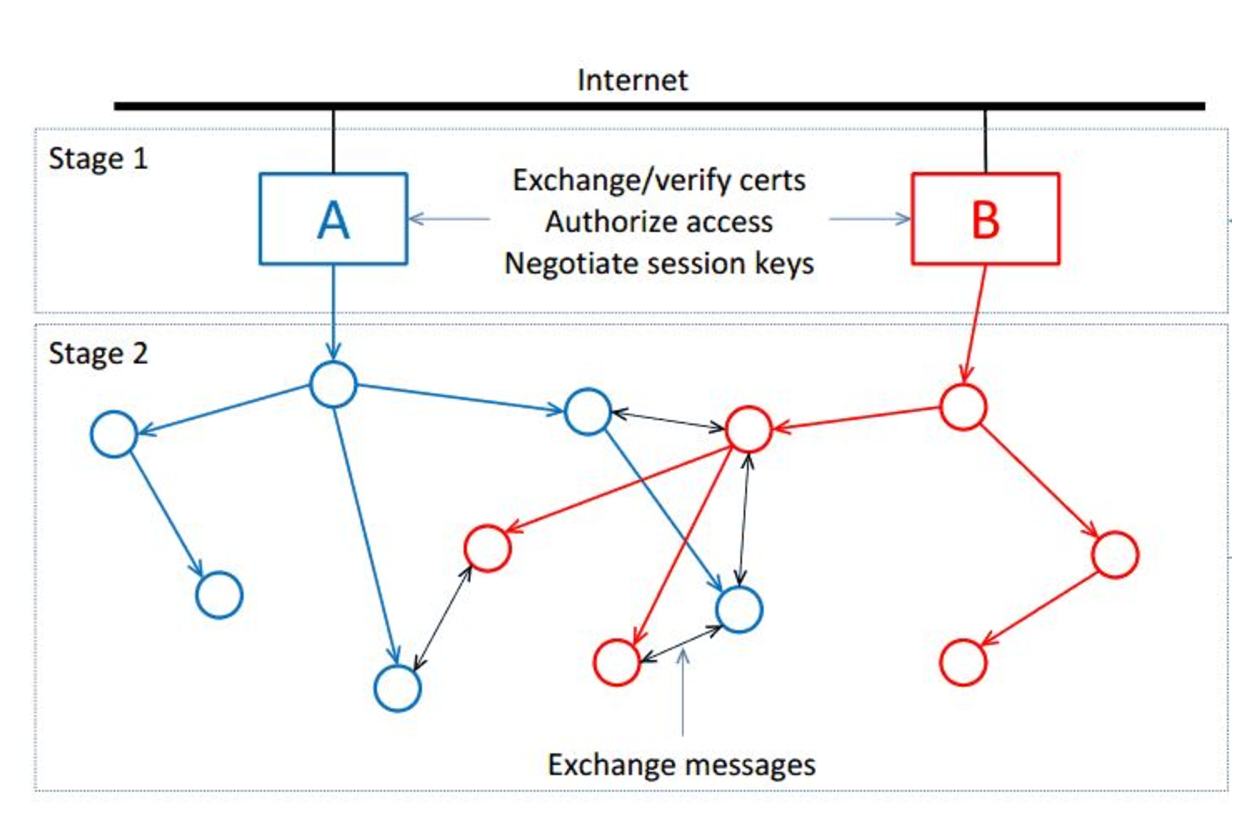
\includegraphics{spartanrpc}

Decreases WSN computational overhead, RAM and ROM consumption. 
\stopslide

%%%%%

\startslide{Results}
\begin{center}
\begin{tabular}{|r||c|c|c|c|} \hline
              & Unsecured & Unstaged* & Staged & Savings\\ \hline
Sensor ROM    &     36254 &    48616 &  36596 & 25\% \\
Sensor RAM    &      2868 &     5417 &   3038 & 44\% \\ \hline
Harvester ROM &     24316 &    35834 &  24436 & 32\% \\
Harvester RAM &      2274 &     4771 &   2402 & 50\% \\ \hline
\end{tabular}
\end{center}
\begin{citemize}
\item Security model: Two different Harvester ``nodes''
\begin{cenumerate}
\item Data download only.
\item Data download and control.
\end{cenumerate}
\end{citemize}
\vspace{0.75in}
{\small * Chapin, Skalka; \textit{SpartanRPC}; Technical Report;
  \url{http://www.cs.uvm.edu/~skalka/skalka-pubs/chapin-skalka-spartanrpctr.pdf}}
\stopslide

%%%%%

\startslide{Future Work}
\begin{citemize}
\item Clarifying ``middle ground'' between language borders.
\item Syntactic transformations: Allowing more natural syntax in Scalaness programs.
\item Incorporating network communication. 
\item Other applications: Backcasting and evolving control.
\end{citemize}
\stopslide

%%%%%

\startslide{Questions?}
\makeatletter
\center{Peter Chapin \textless pchapin@cs.uvm.edu\textgreater}
\center{\cemph{http://tinyurl.com/a85z8cu}}
\makeatother
\stopslide

%%%%%

\startslide{\fml\ Foundations} The \fml\ language\footnote{\cref{Yu David Liu, Christian Skalka,
    and Scott Smith. Type-Specialized Staged Programming with Process Separation. Journal of
    Higher Order and Symbolic Computation, 24(4):341-385, 2012.}} was developed to study these
elements at a foundational level.
\begin{citemize}
\item MetaML-like syntax and semantics, but novel features to moderate interactions between
  separate process spaces.
\item Comprises $F_{\le}$.
\item Resricted form of type construction (not full $\lambda_\omega$).
\item Formal metatheory includes cross-stage type safety---residue of partial evaluation of
  well-typed code is guaranteed to be well-typed.
\end{citemize}
\stopslide

%%%%%

\startslide{Sample Scalaness Typing}
$$
\jmodt{\Delta_1}{\margs{\Delta_2, \Gamma}\lc 
  \imports; \exportsty \rc}
$$
Module type form, where:
\begin{citemize}
\item $\Delta_2$, $\Gamma$ type parameter bounds and term parameter types.
\item $\imports$, $\exportsty$ import and export type signatures.
\item $\Delta_1$ bounds of types constructed externally to the module.
\begin{citemize}
\item Early substitution of these types unsound due to possible contravariant use in $\imports;
  \exportsty$.
\end{citemize}
\end{citemize}
$$
\inferrule[ModInstT]
{\Gamma \vdash \tt{e} : \jmodt{\varnothing}{\margs{\vect{t} \subtype \vect{\t}_1; 
 \vect{x} : \vect{\t}_2} \lc \imports; \exportsty \rc} \\
 \Gamma \vdash \ttvec{s} : \jinst{MetaType}{\ttvec{T}_1} \\
 \Gamma \vdash \ttvec{e}_2 : \ttvec{T}_2 \\
 \vdash \codt{\ttvec{T}_1} \subtype \vect{\t}_1 \\
 \vdash \codt{\ttvec{T}_2} \subtype \vect{\t}_2
}
{\Gamma \vdash \jinst{e}{\ttvec{s}; \ttvec{e}_2} : \jmodt{\ttvec{s} \subtype
    \codt{\ttvec{T}_1}}{\margs{} \lc \imports[\ttvec{s}/\vect{t}]; \exportsty[\ttvec{s}/\vect{t}] \rc} }
$$
\stopslide
